\chapter*{Introduction}

Software development requires thinking about several
dimensions simultaneously. For large programs, writing the actual
computer instructions is not as difficult as figuring out the
details of what the computer is supposed to do. After analyzing what is
needed, program design brings together the data structures, algorithms,
objects, and interactions that accomplish the required tasks. Despite
the importance of analysis and design, programming is still the central
act of software development for several reasons. The weak form of the
\index{Sapir-Whorf}Sapir-Whorf hypothesis suggests that the programming
language we use steers and guides the way we think about software, so
it affects our designs. Software designs are mathematical theorems,
while programs are proofs that test those designs. As in other
branches of mathematics, the proofs reign supreme. In addition, a
correct design can be foiled by an inferior implementation.

This book is a guide and reference for an exciting
programming language called Unicon that has something to offer both
computer scientists as well as casual programmers. You
will find explanations of fundamental principles, unique language
idioms, and advanced concepts and examples. Unicon exists within the
broader context of software development, so the book also covers
software engineering fundamentals. Writing a correct, working
program is the central task of software engineering. This does not
happen automatically as a result of the software design process. Make
no mistake: if you program very much, the programming language you use
is of vital importance. If it weren't, we would still
be programming in machine language.

\section*{Prototyping and the Spiral Model of Development}

A software \index{prototype}prototype is a working subset of a software
system. Prototypes help check software designs and user
interfaces, demonstrate key features to customers, or prove the
feasibility of a proposed solution. A prototype may generate
customer feedback on missing functionality, provide insight on how to
improve the design, lead to a decision about whether to go ahead with a
project or not, or form a starting point for the algorithms and data
structures that will go into the final product. Prototyping is done
early in the software development process. It fits naturally into the
\index{spiral model}\textit{spiral model} of development proposed by
\index{Boehm, Barry}Barry Boehm (1988). Figure I-1 shows the spiral
model; time is measured by the distance from the center. Analysis,
design, coding, and evaluation are repeated to produce a better product
with each iteration. "Prototyping" is the
act of coding during those iterations when the software is not yet
fully specified or the program does not yet remotely implement the
required functionality.

\begin{center}
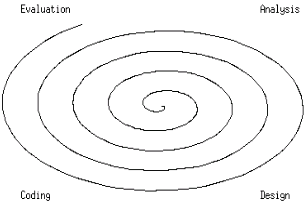
\includegraphics[width=2.5402in,height=1.6799in]{ub-img/ub-img4.png}
\end{center}

{\sffamily\bfseries Figure I-1}
{\sffamily The Spiral Model of Software Development}

\bigskip

\textit{Tight} spirals are better than loose spirals. The more powerful
the prototyping tools, the less time and money spent in early
iterations of development. This translates into either faster
time to market, or a higher quality product. Some prototypes are thrown
away once they have served the purpose of clarifying requirements or
demonstrating some technique. This is OK, but in the spiral model some
prototypes are gradually enhanced until they become the final
production system.

\section*{Icon: a Very High Level Language for Applications}

Icon is a \index{very high-level language}programming language developed
at the University of Arizona. Icon generalizes its developers' experience
creating an earlier language, \index{SNOBOL4}SNOBOL4. Icon
embodies seminal research ideas, but it is also more fun and
easier to program than other languages.  Most very high-level
languages revel in cryptic syntax, while Icon
is not just more powerful, but often more
\textit{readable} than its competitors. This
gain in expressive power without losing readability is an
addicting result of Icon's elegant design.

The current Arizona Icon, version 9.5, is described in
\textit{The Icon Programming Language}, \textit{3rd edition} by Ralph
and Madge Griswold (1996). Its reference implementation is a
virtual machine interpreter. Icon evolved through many releases
over two decades and is far more capable than it was originally. It is
apparently a finished work.

\section*{Enter Unicon: More Icon than Icon}

The name ``Unicon'' refers to the descendant of
Icon described in this book and
distributed from \url{www.unicon.org}.  Unicon is
Icon with portable, platform-independent access to hardware and
software features that have become ubiquitous in modern
applications development, such as objects, networks, and databases.
Unicon is created from the same public domain source code that Arizona
Icon uses, so it has a high degree of compatibility. We were not
free to call it version 10 of the Icon
language, since it was not produced or endorsed by the Icon Project at
the University of Arizona.

Just as the name Unicon frees the Icon Project of all responsibility for
our efforts, it frees us from the requirement of backward
compatibility. While Unicon is almost entirely backward compatible
with Icon, dropping full
compatibility allows us to clear out some dead wood and more
importantly, to make some improvements in the operators that will
benefit everyone at the expense of...no one but the compatibility
police.
This book covers the features of Icon and Unicon together. A
compatibility check list and description of the differences
between Icon and Unicon are given in Appendix D.

\section*{The Programming Languages Food Chain}

It is interesting to compare Icon and Unicon with the competition.
Mainstream programming languages
such as C, C++, and \index{Java}Java, like the assembler languages that
were mainstream before them, are ideal tools
for writing all sorts of programs, so long as vast amounts of
programmer time are available. Throwing more programmers at a big
project does not work well, and programmers are getting more expensive
while computing
resources continue to become cheaper. These pressures
inexorably lead to the use of higher-level languages and the
development of better design and development methods. Such human
changes are incredibly slow compared to technological changes, but they
are visibly occurring nevertheless. Today, the most
productive programmers are using extra CPU cycles and memory
to reduce the time it takes to develop useful programs.

There is a subcategory of mainstream languages, marketed as \index{rapid
application development}\textit{rapid application development}
languages, whose stated goals seem to address this phenomenon.
Languages such as \index{Visual Basic}Visual Basic or
\index{PowerBuilder}PowerBuilder provide
graphical interface builders and integrated database connectivity,
giving productivity increases in the domain of data entry and
presentation. The value added in these products are in their
programming environments, not their languages. The \index{integrated
development environment}integrated development environments and tools
provided with these languages are to be acclaimed and emulated, but
they do not provide productivity gains that are equally relevant to all
application domains. They are only a partial solution to the needs of
complex applications.

Icon is designed to be easier and faster to program than mainstream
languages. The value it adds is in the expressive power of the language
itself, in the category of very high level languages
that includes \index{Lisp}Lisp,
\index{APL}APL, \index{Smalltalk}Smalltalk, \index{REXX}REXX,
\index{Perl}Perl, \index{Tcl}Tcl, \index{Python}Python, and
\index{Ruby}Ruby; there are
many others. Very high-level languages can be subdivided into
\index{scripting languages}scripting languages and applications
languages. Scripting languages often glue programs
together from disparate sources. They are typically strong in areas
such as multilingual interfacing and file system interactions, while
suffering from weaker expression semantics, typing, scope rules, and
control structures than their applications-oriented cousins.
Applications languages typically originate within a particular
application domain and support that domain with special syntax, control
structures, and data types. Since scripting \textit{is} an application
domain, scripting languages are just one prominent
subcategory of very high-level languages.

Icon is an applications language with roots in text
processing and linguistics. Icon programs tend to be more readable than
similar programs written in other very high-level languages, making
Icon well-suited to the aims of \index{literate
programming}\textit{literate programming}. For example, Icon was used
to implement Norman Ramsey's literate
programming tool \texttt{noweb} (Ramsey, 1994). Literate programming is
the practice of writing programs and their supporting textual
description together in a single document.

Unicon makes the core contributions of Icon useful
for a broader range of applications. This book's many
examples illustrate the range of tasks for which Unicon is well
suited, and these examples are the evidence in
support of Unicon's existence.
Consider using Unicon when one or more of the following conditions are
true. The more conditions that are true, the more you will
benefit from Unicon.
\begin{itemize} \itemsep0pt
\item Programmer time must be minimized.
\item Maintainable, concise source code is desired.
\item The program includes complex data structures or experimental
      algorithms.
\item The program involves a mixture of text processing and analysis, custom
      graphics, data manipulation, network or file system operations.
\item The program must run on several operating systems and have a
      nearly identical graphical user interface with little or no source code
      differences.
\end{itemize}
Unicon is not the last word in programming. You probably should not use
Unicon if your program has one or more of the following requirements:
\begin{itemize} \itemsep0pt
\item The fastest possible performance is needed.
\item The program has hard real-time constraints.
\item The program must perform low-level or platform-specific
      interactions with the hardware or operating system.
\end{itemize}
Programming languages play a key role in software development.
The Unicon language is a very high level
\index{object-oriented programming}object-oriented language
with a unique combination of expressive power and scalable rapid
development. In this book, many examples from a wide range
of application areas demonstrate how to apply and combine Unicon's
language constructs to solve real-world problems.
It is time to move past the introductions. Prepare to be spoiled by
this language. You may have the same feelings that
Europeans felt when they gave up using Roman numerals and
switched to the Hindu-Arabic number system. ``This
multiplication stuff isn't that hard anymore!''
